\section{Data translation}
\subsection{Data collection}
In order to collect suitable data we tried different data service providers such as Datahub, finally we have collected total four datasets from three different sources and in three different formats, including: 

%For each subsubsection below:
%Which format did the data have? CSV, JSON, XLSX?
%Size of each dataset? (how many entities)
%Which attributes were collected for each dataset? 
%Why? Optional ones? Nonoptional ones? Resulting sparsity of each attribute?
%How did collect each dataset? Queries (give an excerpt), downloads...




\subsubsection{Forbes: Company}
%Silvia/Zehui
The Forbes offers a .xls file with a list of Top 2000 companies during the period 2000 to 2014 which were published in Forbes magazine because of great performance in terms of business achievements. This dataset describes the basic information about these top 2000 companies. For example, location shows where this company is founded, industry depicts what fields the company focus on and so on.
\subsubsection{DBpedia: Company }
The information of company is extracted from DBpedia, since it provides relatively complete information.  To access information from DBPedia we used the public SPARQL endpoint (at http://dbpedia.org/sparql). Figure 1.1 is our query for company, actually there is total 764398 companies in DBpedia, which would be too much for us and also not easy to handle it in terms of processing time and space. In order to reduce the number of data, we limit the company types to "company" and "public company" and only extract the companies that provide attributes "LocationCity" and "LocationCountry", these two attributes can also be related with Location Information, that's why we consider them as necessary and others are optional. On the other hand, if all these attributes are necessary, there will be only few thousands companies extracted, because not all companies have all these nine attributes, in this case few overlapping data will be in the final integration results. In addition to this, as many attributes such as KeyPeople, locationCity have multiple values which result in the same company would appear more than one times, to avoid these duplicates we used "group\_contac", a function in Sparql, to group many value together. There are also many values for Revenue but without date notation, so we just took the maximum value. 

\subsubsection{Freebase: Company}
%Yiru
Freebase, like DBPedia, offers a web service which can be queried for data. Instead of SPARQL, however, the service is used by sending JSON requests. Like DBPedia this lets us select certain companies, or companies with certain attributes.


\subsubsection{DBpedia: Location}
%Silvia/Zehui
We also extracted Location information from DBpedia with the same method as Company. Figure 1.2 is the query for location. For the same reason as Company, we limit the location types to "city" and "AdministrativeRegion", which are more relevant to our company dataset. Also some attributes have many values without extra information, it's hard to identify which one represents the current state, thus, we just took the maximum number of them among multiple values. Furthermore, the name of locations are provide in different languages, while in our project we just focus on english, so we filtered language as english.


\begin{table}[htb]
\centering
\caption{Basic Profile of Each Dataset}
\label{my-label}
\begin{tabular}{|c|c|c|c|c|c|}
\hline
\multicolumn{1}{|l|}{}         & \multicolumn{1}{l|}{Source} & \multicolumn{1}{l|}{Format} & \multicolumn{1}{l|}{Class} & \multicolumn{1}{l|}{\#Entities} & \multicolumn{1}{l|}{\#Attributes} \\ \hline
                               & \multicolumn{5}{c|}{List of Attributes}                                                                                                                      \\ \hline
\multirow{Forbes Global} & forbes.com                  & xlsx                        & company                    & 2000                            & 7                                 \\ \cline{2-6} 
                               & \multicolumn{5}{c|}{Company,country,industry,revenue,assets,marketvalue,profit}                                                                              \\ \hline
\multirow{DBpedia}       & dbpedia.org/sparql          & csv                         & company                    & 16051                           & 9                                 \\ \cline{2-6} 
                               & \multicolumn{5}{c|}{\begin{tabular}[c]{@{}c@{}}Company,country,industry,revenue,numberOfemployees,\\ foundingYear,assets,keyPeople,location\end{tabular}}    \\ \hline
\multirow{Freebase}      & freebase.com/query          & json                        & company                    &                                 & 9                                 \\ \cline{2-6} 
                               & \multicolumn{5}{c|}{\begin{tabular}[c]{@{}c@{}}Company,country,industry,revenue,numberOfemployees,\\ foundingYear,profit,keyPeople,location\end{tabular}}    \\ \hline
\multirow{Dbpeida}       & dbpedia.org/sparql          & csv                         & location                   & 3270                            & 5                                 \\ \cline{2-6} 
                               & \multicolumn{5}{c|}{Location,country,population,area,elevation}                                                                                              \\ \hline
\end{tabular}
\end{table}







\subsection{Integrated schema}
%Take from data\ForbesPlan\Forbes-integrated schema.docx
We looked into four datasets and did the following Integrated Schema.In this table we use prefix dataset 1, 2, 3,4 respectively represent Forbes, DBpedia(company), Freebase and DBpedia(Location)

\begin{table}[h]
\centering
\caption{Integrated Schema}
\label{my-label}
\begin{tabular}{|c|c|c|c|}
\hline
Class Name & Attributes Name & \begin{tabular}[c]{@{}c@{}}Datasets in which \\ attribute is found\end{tabular} & \begin{tabular}[c]{@{}c@{}}Conflict resolution\\        strategies\end{tabular} \\ \hline
company & (company)name & dataset 1, 2, 3 & \begin{tabular}[c]{@{}c@{}}LongestString, \\ FavourSources, \\ Voting\end{tabular} \\ \hline
company,location & country & dataset 1, 2, 3, 4 & Voting \\ \hline
company & industries & dataset 1, 2, 3 & Union \\ \hline
company & \begin{tabular}[c]{@{}c@{}}Sales/\\ revenue\end{tabular} & dataset 1, 2, 3 & FavourSources \\ \hline
company & \begin{tabular}[c]{@{}c@{}}number Of \\ Employees\end{tabular} & dataset 2, 3 & \begin{tabular}[c]{@{}c@{}}Average,\\ Growth: Max\end{tabular} \\ \hline
company & \begin{tabular}[c]{@{}c@{}}founding year/ \\ date founded\end{tabular} & dataset 2, 3 & \begin{tabular}[c]{@{}c@{}}MostComplete\\ (complete date) \\ AND,\\ MostComplete \\ (sample)\end{tabular} \\ \hline
company & Assets & dataset 1, 2 & FavourSources \\ \hline
company & Market Value & dataset 1 & / \\ \hline
company & profit & dataset 1, 3 & FavourSources \\ \hline
company & continent & dataset 1 & / \\ \hline
company & \begin{tabular}[c]{@{}c@{}}keyPeople/\\  leadership\end{tabular} & dataset 2, 3 & Union \\ \hline
\begin{tabular}[c]{@{}c@{}}company,\\ location\end{tabular} & name & dataset 2, 3, 4 & \begin{tabular}[c]{@{}c@{}}Union AND \\ FavourSources\end{tabular} \\ \hline
location & \begin{tabular}[c]{@{}c@{}}population\\ total\end{tabular} & dataset 4 & / \\ \hline
location & area total & dataset 4 & / \\ \hline
location & elevation & dataset 4 & / \\ \hline
\end{tabular}
\end{table}


\subsection{Data transformations}
In this phase, two kinds of transformations occurred. One is processed during mapping, another one is processed with Java Programming. First of all, during mapping process, since revenue and assets are written in scientific notation, while in our target schema it should be in original data, therefore we used some functions in Mapforce to convert scientific notation into decimals. Secondly, the original data has no ID, but it will be used later, so we also append "ID" for these four dataset individually with "GenerateID" function provided by MapForce.
In addition, many attributes in Dbpedia are in the form of URL, while only the values are meaningful, thus, we removed the URL part with Java and extracted values we want, in the mean time, we also replaced punctuation and symbols like "\_" or ".". Furthermore, some words, that have various spellings such as US, USA, U.S, America, were replaced with unified ?United States of America?.


\begin{figure}[H]
	\begin{center}
	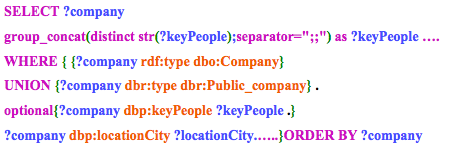
\includegraphics[width=10cm]{DB_Com}
	\caption[DBpedia Query For Company]{DBpedia Query For Company}
	\label{fig:db}
	\end{center}
\end{figure}


\begin{figure}[H]
	\begin{center}
	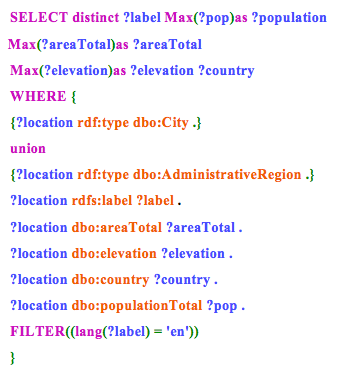
\includegraphics[width=10cm]{DB_Loc}
	\caption[DBpedia Query For Location]{DBpedia Query For Location}
	\label{fig:db}
	\end{center}
\end{figure}
%Oliver
%Which attributes did we transform in which way? 
%Also: Example for each transformation showing why we did it
%DBpedia values: Very often URL
%Company and location names: Removed common strings that are inconsistent among datasets, e.g. Apple / Apple, Inc.
% 	also: Replaced punctuation and symbols like "_" or "."
%	Result example: Apple (Forbes) <-> Apple,_Inc (DBpedia)
%Countries: Replaced different spellings of same word 
%	e.g. US, USA, U.S., America with "United States of America" or UK, England with United Kingdom
%Numeric attributes to do with money: Scientific notation, small values from Forbes
%	e.g. 1.17E+10 ==> 11.700.000.000
% 	e.g. 483,1 (Apple in Forbes) ==> 483.100.000.000




